\PassOptionsToPackage{unicode=true}{hyperref} % options for packages loaded elsewhere
\PassOptionsToPackage{hyphens}{url}
%
\documentclass[10pt,ignorenonframetext,]{beamer}
\usepackage{pgfpages}
\setbeamertemplate{caption}[numbered]
\setbeamertemplate{caption label separator}{: }
\setbeamercolor{caption name}{fg=normal text.fg}
\beamertemplatenavigationsymbolsempty
% Prevent slide breaks in the middle of a paragraph:
\widowpenalties 1 10000
\raggedbottom
\setbeamertemplate{part page}{
\centering
\begin{beamercolorbox}[sep=16pt,center]{part title}
  \usebeamerfont{part title}\insertpart\par
\end{beamercolorbox}
}
\setbeamertemplate{section page}{
\centering
\begin{beamercolorbox}[sep=12pt,center]{part title}
  \usebeamerfont{section title}\insertsection\par
\end{beamercolorbox}
}
\setbeamertemplate{subsection page}{
\centering
\begin{beamercolorbox}[sep=8pt,center]{part title}
  \usebeamerfont{subsection title}\insertsubsection\par
\end{beamercolorbox}
}
\AtBeginPart{
  \frame{\partpage}
}
\AtBeginSection{
  \ifbibliography
  \else
    \frame{\sectionpage}
  \fi
}
\AtBeginSubsection{
  \frame{\subsectionpage}
}
\usepackage{lmodern}
\usepackage{amssymb,amsmath}
\usepackage{ifxetex,ifluatex}
\usepackage{fixltx2e} % provides \textsubscript
\ifnum 0\ifxetex 1\fi\ifluatex 1\fi=0 % if pdftex
  \usepackage[T1]{fontenc}
  \usepackage[utf8]{inputenc}
  \usepackage{textcomp} % provides euro and other symbols
\else % if luatex or xelatex
  \usepackage{unicode-math}
  \defaultfontfeatures{Ligatures=TeX,Scale=MatchLowercase}
\fi
\usefonttheme{serif}
% use upquote if available, for straight quotes in verbatim environments
\IfFileExists{upquote.sty}{\usepackage{upquote}}{}
% use microtype if available
\IfFileExists{microtype.sty}{%
\usepackage[]{microtype}
\UseMicrotypeSet[protrusion]{basicmath} % disable protrusion for tt fonts
}{}
\IfFileExists{parskip.sty}{%
\usepackage{parskip}
}{% else
\setlength{\parindent}{0pt}
\setlength{\parskip}{6pt plus 2pt minus 1pt}
}
\usepackage{hyperref}
\hypersetup{
            pdftitle={A Bayesian Model of Memory for Text},
            pdfborder={0 0 0},
            breaklinks=true}
\urlstyle{same}  % don't use monospace font for urls
\newif\ifbibliography
\usepackage{longtable,booktabs}
\usepackage{caption}
% These lines are needed to make table captions work with longtable:
\makeatletter
\def\fnum@table{\tablename~\thetable}
\makeatother
\setlength{\emergencystretch}{3em}  % prevent overfull lines
\providecommand{\tightlist}{%
  \setlength{\itemsep}{0pt}\setlength{\parskip}{0pt}}
\setcounter{secnumdepth}{0}

% set default figure placement to htbp
\makeatletter
\def\fps@figure{htbp}
\makeatother

\makeatletter
\let\@@magyar@captionfix\relax
\makeatother

\RequirePackage{pifont,manfnt}
\RequirePackage{booktabs}
\RequirePackage[T1]{fontenc}
\RequirePackage{mathpazo}
\RequirePackage{eulervm}
\RequirePackage{tikz}
\linespread{1.05}
\RequirePackage{xspace}
\RequirePackage{apacite}
\RequirePackage{rotating}
\RequirePackage{multirow}
\usepackage{fontawesome}
\usepackage{nth}

\newcommand{\Prob}[1]{\mathrm{P}( #1 )}
\newcommand{\dcat}[1]{\mathrm{dcat}( #1 )}
\newcommand{\ddirichlet}[1]{\mathrm{ddirichlet}( #1 )}
\newcommand*{\given}{\vert}
\newcommand{\hdpmm}{\textsc{hdptm}\xspace}
\newcommand{\bnc}{\textsc{bnc}\xspace}

\newcommand\iidsim{\mathrel{\overset{\makebox[0pt]{\mbox{\normalfont\tiny iid}}}{\sim}}}
\newcommand\defeq{\mathrel{\overset{\makebox[0pt]{\mbox{\normalfont\tiny def}}}{=}}}
\newcommand{\hpd}{\textsc{hpd}\xspace}
\newcommand{\Probc}[1]{\mathrm{P}_{\text{\!\tiny \textsc{c}}}( #1 )}
\newcommand{\Proba}[1]{\mathrm{P}_{\text{\!\tiny \textsc{a}}}( #1 )}
\newcommand{\wnew}{w_{j}}
\newcommand{\wjinew}{w_{ji}}
\newcommand{\pinew}{\pi_{j}}
\newcommand{\data}{\mathcal{D}}
\newcommand{\dic}{\textsc{dic}\xspace}

\setbeamerfont{title}{family=\it}
\setbeamerfont{frametitle}{family=\it}

\RequirePackage{tikz}
\usetikzlibrary{trees}
\usetikzlibrary{matrix}

\RequirePackage{amssymb,latexsym,amsmath,amsfonts,amscd}

\usecolortheme[named=gray]{structure} 
\setbeamercolor{titlelike}{fg=black!60!red}
\definecolor{Mygrey}{gray}{0.75}

\newcommand{\rreallytiny}{\fontsize{3}{3}\selectfont}
\newcommand{\reallytiny}{\fontsize{5}{5}\selectfont}

\usetikzlibrary{decorations.pathmorphing} % noisy shapes
\usetikzlibrary{fit}					% fitting shapes to coordinates
\usetikzlibrary{backgrounds}	% drawing the background after the foreground
\usetikzlibrary{matrix}

\tikzstyle{background}=[rectangle, fill=none,
						draw=black,
                                                inner sep=0.3cm,
                                                rounded corners=3mm]

\tikzstyle{observation}=[circle,font=\small,minimum size=5mm,inner sep=0mm,
                                    draw=black!70,
                                    fill=black!10]

\tikzstyle{state}=[circle,font=\small,minimum size=5mm,inner sep=0mm,
                                   draw=black!70,
                                    fill=none]

\tikzstyle{limit}=[rectangle,font=\small,minimum size=0mm,inner sep=0mm,
                                    fill=none]

\tikzstyle{parameter}=[circle,font=\small,minimum size=5mm,inner sep=0mm,
                                   draw=black!70,
                                    fill=none]


\graphicspath{{../images/}}

\DeclareSymbolFont{legacymaths}{OT1}{cmr}{m}{n}
\DeclareMathAccent{\dot}     {\mathalpha}{legacymaths}{95}
\DeclareMathAccent{\bar}     {\mathalpha}{legacymaths}{22}
\DeclareMathAccent{\tilde}     {\mathalpha}{legacymaths}{126}

\title{A Bayesian Model of Memory for Text}
\author{Mark Andrews\\
Psychology Department, Nottingham Trent University\\
~\\
\faEnvelopeO~ \texttt{mark.andrews@ntu.ac.uk}\\
\faTwitter~\texttt{@xmjandrews}\\
\faGithub~\texttt{https://github.com/lawsofthought/bps-cog-2018}}
\date{August 30, 2018}

\begin{document}
\frame{\titlepage}

\begin{frame}{Memory for text}
\protect\hypertarget{memory-for-text}{}

\begin{itemize}
\tightlist
\item
  The seminal study on memory for text is usually attributed to Bartlett
  (1932).
\item
  From this, and schema based accounts of text memory (see, e.g., Bower,
  Black, \& Turner, 1979), there has been something close to a consensus
  on the broad or general characteristics of human text memory.
\item
  According to this general account --- which we can summarize by the
  following schematic:

  \begin{center}
  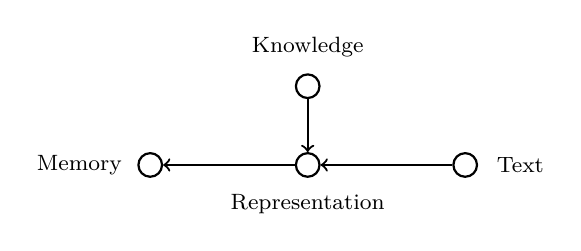
\begin{tikzpicture}[thick]
  \tikzstyle{lables}=[font=\footnotesize]
  \node (knowledge) at (0,2) [inner sep=0pt,minimum size=3mm,circle,draw] {};
  \node (representation) at (0,1) [inner sep=0pt,minimum size=3mm,circle,draw] {};
  \node (text) at (2,1) [inner sep=0pt,minimum size=3mm,circle,draw] {};
  \node (memory) at (-2,1) [inner sep=0pt,minimum size=3mm,circle,draw] {};
  \draw [->] (knowledge) -- (representation);
  \draw [->] (text) -- (representation);
  \draw [->] (representation) -- (memory);
  \node[lables] (representationlabel) at (0,.5) {Representation};
  \node[lables] (knowledgelabel) at (0,2.5) {Knowledge};
  \node[lables] (textlabel) at (2.7,1) {Text};
  \node[lables] (memorylabel) at (-2.9,1) {Memory};
  \end{tikzpicture}
  \end{center}

  --- the recognition or recall of items in a text is based on querying
  a representation of the text that is built up on the basis of
  background knowledge and experience.
\end{itemize}

\end{frame}

\begin{frame}{Probabilistic account of memory for text}
\protect\hypertarget{probabilistic-account-of-memory-for-text}{}

\begin{itemize}
\tightlist
\item
  We begin with the assumption that our background knowledge that is
  relevant for our memory of text is knowledge of the distributional
  statistics.
\item
  Given a probabilistic language model, we may use Bayes's rule to infer
  the statistical patterns inherent in any given text.\\
\item
  We may then predict, via posterior predictive inference, the words are
  and are not typical of this inferred statistical representation.
\item
  As such, this provides a computational description of the previous
  schematic, i.e.,

  \begin{center}
  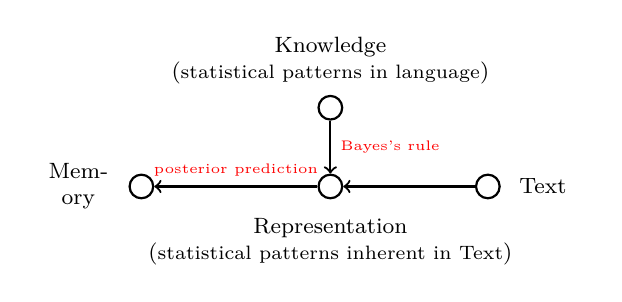
\begin{tikzpicture}[thick,node distance=6mm]
  \tikzstyle{lables}=[font=\footnotesize,text width=15em,text centered]
  \node (knowledge) at (0,2) [inner sep=0pt,minimum size=3mm,circle,draw] {};
  \node (representation) at (0,1) [inner sep=0pt,minimum size=3mm,circle,draw] {};
  \node (text) at (2,1) [inner sep=0pt,minimum size=3mm,circle,draw] {};
  \node (memory) at (-2.4,1) [inner sep=0pt,minimum size=3mm,circle,draw] {};
  \draw [->] (knowledge) -- (representation) node[red,right,midway] {{\tiny Bayes's rule}};
  \draw [->] (text) -- (representation);
  \draw [->] (representation) -- (memory) node[red,above,midway] {{\tiny posterior prediction}};
  \node[lables] (representationlabel) at (0,.3) {Representation  \\ ({\scriptsize statistical patterns inherent in \emph{Text}})};
  \node[lables] (knowledgelabel) [above of=knowledge] {Knowledge \\ ({\scriptsize statistical patterns in language})};
  \node[lables, text width=3em] (textlabel) at (2.7,1) {Text};
  \node[lables, node distance=8mm, text width=3em] (memorylabel) [left of=memory] {Memory};
  \end{tikzpicture}
  \end{center}
\end{itemize}

\end{frame}

\begin{frame}{Probabilistic topic models}
\protect\hypertarget{probabilistic-topic-models}{}

\begin{itemize}
\tightlist
\item
  \emph{Probabilistic topic models} (see, e.g., Griffiths, Steyvers, \&
  Tenenbaum, 2007) have proved effective in capturing the statistical
  patterns that characterize coarse-grained ``discourse topics''.
\item
  Topic models model each word in a text as a sample from one of many
  underlying probability distributions over a vocabulary.
\item
  For example, here is a sample of 6 topics from an inferred model:
\end{itemize}

\centering\small 
\begin{tabular}{cccccc}
theatre &    music &  league & prison & rate & pub           \\
stage &      band &   cup & years & cent & guinness          \\
arts &       rock &   season & sentence & inflation & beer \\
play &       song &   team & jail & recession & drink        \\
dance &      record & game & home & recovery & bar           \\
opera &      pop &    match & prisoner & economy & drinking  \\
cast &       dance &  division & serving & cut & alcohol     \\
\end{tabular}\normalsize

\begin{itemize}
\tightlist
\item
  In this study, we used a \emph{Hierarchical Dirichlet process topic
  model} (\hdpmm), which is a non-parametric probabilistic topic model.
\end{itemize}

\end{frame}

\begin{frame}{Inference and predictions in topic models}
\protect\hypertarget{inference-and-predictions-in-topic-models}{}

\begin{itemize}
\item
  Given this model, we obtain a formal model of background knowledge,
  text representation, and recall or recognition memory:

  \begin{itemize}
  \tightlist
  \item
    \emph{Background knowledge}: From a corpus of example texts, we can
    infer the posterior distribution over the topics.
  \item
    \emph{Text representation}: For any given text, we can infer how
    well it is characterized by each inferred topic.
  \item
    \emph{Memory}: Given the text representation, we can then predict
    which words are typical or expected on the basis of that inferred
    representation.
  \end{itemize}
\item
  More formally, having inferred topics, given a new text \(\wnew\), we
  infer the posterior probability over \(\pinew\), which is the
  probability distribution over the discourse topics in \(\wnew\). We
  then use the posterior predictive distribution to infer the words that
  are typical of the topics inherent in \(\wnew\): \[
    \Prob{\wjinew \given \wnew,\data} = \int \Prob{\wjinew \given \pinew, \data}\Prob{\pinew \given \wnew, \data} d\pinew
  \]
\end{itemize}

\end{frame}


\begin{frame}{Example text 1: Posterior predictions}

	{\small\textit{
Improve your mood and counteract stress: Ask anyone who exercises regularly and
they will tell you that they always feel exhilarated at the end of a session —
even if they had begun by feeling that they were not in the mood for exercise
and had almost forced themselves to continue. Physical fitness also provides
considerable protection against stress and the illnesses it can cause\ldots maintain an already high level of stress.
    }}
    \begin{center}
{\fontsize{7.29}{30}\selectfont \textit{relaxation}}
{\fontsize{13.42}{30}\selectfont feel}
{\fontsize{9.62}{30}\selectfont \textit{mind}}
{\fontsize{29.68}{30}\selectfont exercise}
{\fontsize{10.34}{30}\selectfont \textit{people}}
{\fontsize{6.97}{30}\selectfont \textit{exercising}}
{\fontsize{7.55}{30}\selectfont \textit{stretching}}
{\fontsize{18.49}{30}\selectfont \textit{walking}}
{\fontsize{10.00}{30}\selectfont \textit{stamina}}
{\fontsize{7.45}{30}\selectfont \textit{build}}
{\fontsize{6.81}{30}\selectfont \textit{energy}}
{\fontsize{11.55}{30}\selectfont \textit{routine}}
{\fontsize{16.41}{30}\selectfont \textit{walk}}
{\fontsize{8.93}{30}\selectfont \textit{swimming}}
{\fontsize{14.17}{30}\selectfont fit}
{\fontsize{17.36}{30}\selectfont \textit{training}}
{\fontsize{9.10}{30}\selectfont \textit{weight}}
{\fontsize{7.32}{30}\selectfont \textit{aerobics}}
{\fontsize{14.26}{30}\selectfont \textit{health}}
{\fontsize{7.54}{30}\selectfont \textit{yoga}}
{\fontsize{6.66}{30}\selectfont \textit{anxiety}}
{\fontsize{10.48}{30}\selectfont \textit{programme}}
{\fontsize{7.89}{30}\selectfont \textit{rest}}
{\fontsize{7.01}{30}\selectfont session}
{\fontsize{19.44}{30}\selectfont fitness}
{\fontsize{8.89}{30}\selectfont \textit{increase}}
{\fontsize{8.78}{30}\selectfont life}
{\fontsize{8.73}{30}\selectfont \textit{running}}
{\fontsize{9.96}{30}\selectfont \textit{week}}
{\fontsize{8.44}{30}\selectfont \textit{jogging}}
{\fontsize{7.94}{30}\selectfont \textit{rate}}
{\fontsize{7.09}{30}\selectfont level}
{\fontsize{12.18}{30}\selectfont \textit{aerobic}}
{\fontsize{8.87}{30}\selectfont \textit{tension}}
{\fontsize{18.45}{30}\selectfont exercises}
{\fontsize{11.58}{30}\selectfont regular}
{\fontsize{14.47}{30}\selectfont stress}
{\fontsize{7.06}{30}\selectfont \textit{start}}
{\fontsize{7.04}{30}\selectfont \textit{begin}}
{\fontsize{17.27}{30}\selectfont \textit{muscles}}
{\fontsize{6.76}{30}\selectfont \textit{gym}}
{\fontsize{12.26}{30}\selectfont \textit{minutes}}
{\fontsize{11.16}{30}\selectfont mood}
{\fontsize{12.36}{30}\selectfont \textit{heart}}
{\fontsize{11.34}{30}\selectfont \textit{strength}}
{\fontsize{19.97}{30}\selectfont \textit{body}}
{\fontsize{12.18}{30}\selectfont \textit{muscle}}
{\fontsize{16.99}{30}\selectfont physical}
{\fontsize{13.20}{30}\selectfont day}
{\fontsize{17.37}{30}\selectfont time}
    \end{center}
\end{frame}


\begin{frame}{Example text 2: Posterior predictions}

	{\small\textit{
    Developmental norms are an attempt to provide an indication of the ages at which
one might expect ordinary children to show evidence of certain skills or
abilities. Since children vary with respect to the ages at which they
demonstrate any particular behaviour, norms represent an ‘average’ obtained
from an examination of the developmental changes occurring in a large number of
children. Data from a large sample \ldots normally developing children.}
    }
    \begin{center}
    {\fontsize{4.65}{35}\selectfont data}
{\fontsize{11.90}{35}\selectfont \textit{time}}
{\fontsize{4.87}{35}\selectfont \textit{carried}}
{\fontsize{6.02}{35}\selectfont \textit{play}}
{\fontsize{4.64}{35}\selectfont \textit{individual}}
{\fontsize{34.93}{35}\selectfont children}
{\fontsize{7.95}{35}\selectfont \textit{items}}
{\fontsize{14.30}{35}\selectfont \textit{scores}}
{\fontsize{22.39}{35}\selectfont cent}
{\fontsize{9.32}{35}\selectfont \textit{found}}
{\fontsize{4.83}{35}\selectfont \textit{measured}}
{\fontsize{6.39}{35}\selectfont \textit{information}}
{\fontsize{4.61}{35}\selectfont average}
{\fontsize{9.98}{35}\selectfont \textit{school}}
{\fontsize{4.52}{35}\selectfont \textit{samples}}
{\fontsize{11.76}{35}\selectfont sample}
{\fontsize{5.94}{35}\selectfont \textit{extent}}
{\fontsize{14.06}{35}\selectfont \textit{adults}}
{\fontsize{8.25}{35}\selectfont \textit{family}}
{\fontsize{4.49}{35}\selectfont \textit{reliability}}
{\fontsize{6.15}{35}\selectfont \textit{set}}
{\fontsize{7.32}{35}\selectfont \textit{population}}
{\fontsize{5.97}{35}\selectfont behaviour}
{\fontsize{32.47}{35}\selectfont \textit{test}}
{\fontsize{8.77}{35}\selectfont \textit{parent}}
{\fontsize{11.21}{35}\selectfont ability}
{\fontsize{22.31}{35}\selectfont \textit{testing}}
{\fontsize{6.09}{35}\selectfont \textit{aged}}
{\fontsize{8.50}{35}\selectfont \textit{assessment}}
{\fontsize{13.70}{35}\selectfont \textit{adult}}
{\fontsize{12.39}{35}\selectfont \textit{score}}
{\fontsize{5.75}{35}\selectfont \textit{low}}
{\fontsize{7.96}{35}\selectfont \textit{childhood}}
{\fontsize{4.16}{35}\selectfont \textit{increase}}
{\fontsize{4.75}{35}\selectfont \textit{level}}
{\fontsize{5.18}{35}\selectfont \textit{result}}
{\fontsize{7.88}{35}\selectfont provide}
{\fontsize{5.20}{35}\selectfont \textit{scale}}
{\fontsize{9.62}{35}\selectfont performance}
{\fontsize{15.81}{35}\selectfont \textit{tested}}
{\fontsize{20.77}{35}\selectfont \textit{parents}}
{\fontsize{10.22}{35}\selectfont \textit{measure}}
{\fontsize{17.92}{35}\selectfont \textit{results}}
{\fontsize{7.86}{35}\selectfont \textit{mother}}
{\fontsize{16.96}{35}\selectfont age}
{\fontsize{4.77}{35}\selectfont \textit{compared}}
{\fontsize{28.77}{35}\selectfont child}
{\fontsize{5.57}{35}\selectfont \textit{home}}
{\fontsize{9.11}{35}\selectfont \textit{validity}}
{\fontsize{29.15}{35}\selectfont \textit{tests}}
    \end{center}
\end{frame}

\begin{frame}{Training and test corpus}
\protect\hypertarget{training-and-test-corpus}{}

\begin{itemize}
\tightlist
\item
  As our training corpus, we used the British National Corpus (\bnc).
\item
  From the entire \bnc, we extracted approximately 200,000 texts, each
  with between 250 and 500 words.
\item
  This gave a corpus of approximately 80m word tokens, and 50K word
  types.
\item
  We randomly selected exactly 50 texts from the training corpus, and
  removed them.
\item
  Having inferred the topics on the basis of the training corpus, we
  calculated the posterior predictive distribution for each of the 50
  test texts.
\end{itemize}

\end{frame}

\begin{frame}{Comparison models}
\protect\hypertarget{comparison-models}{}

\begin{itemize}
\tightlist
\item
  We compare to predictions made by two \emph{associative} models:

  \begin{enumerate}
  \tightlist
  \item
    From the \bnc, we calculate the conditional probability of \(w_k\)
    and \(w_l\) as follows:
    \[\Probc{w_k \given w_l} = \frac{\Probc{w_k, w_l}}{\Probc{w_l}},\]
    where \(\Probc{w_k, w_l}\) is the co-occurrence probability of
    \(w_k\) and \(w_l\).
  \item
    Using the \emph{small world of word} association norms, we calculate
    conditional probability of word \(w_k\) given \(w_l\) with \[
        \Proba{w_k \given w_l} = \frac{A_{kl}}{\sum_{i=1}^V A_{il}},
        \] where \(A_{kl}\) indicates frequency that word \(w_k\) is
    stated as associated with word \(w_l\).
  \end{enumerate}
\item
  Given a text \(\wnew = w_{j1}, w_{j2} \ldots w_{j n_j}\), these
  models' predictions are: \[
  \Probc{w_k \given \wnew} =\frac{1}{n_j} \sum_{i=1}^{n_{j}} \Probc{w_k \given w_{ji}},\quad
    \Proba{w_k \given \wnew} =\frac{1}{n_j} \sum_{i=1}^{n_{j}} \Proba{w_k \given w_{ji}},
  \]
\end{itemize}

\end{frame}

\begin{frame}{Experiment}
\protect\hypertarget{experiment}{}

\begin{itemize}
\tightlist
\item
  216 people (113 female, 103 male) participated in the experiment.
\item
  Each participant read three randomly chosen texts (from the set of
  50).
\item
  Their memory was tested with either a recall or a recognition test.
\end{itemize}

\begin{center}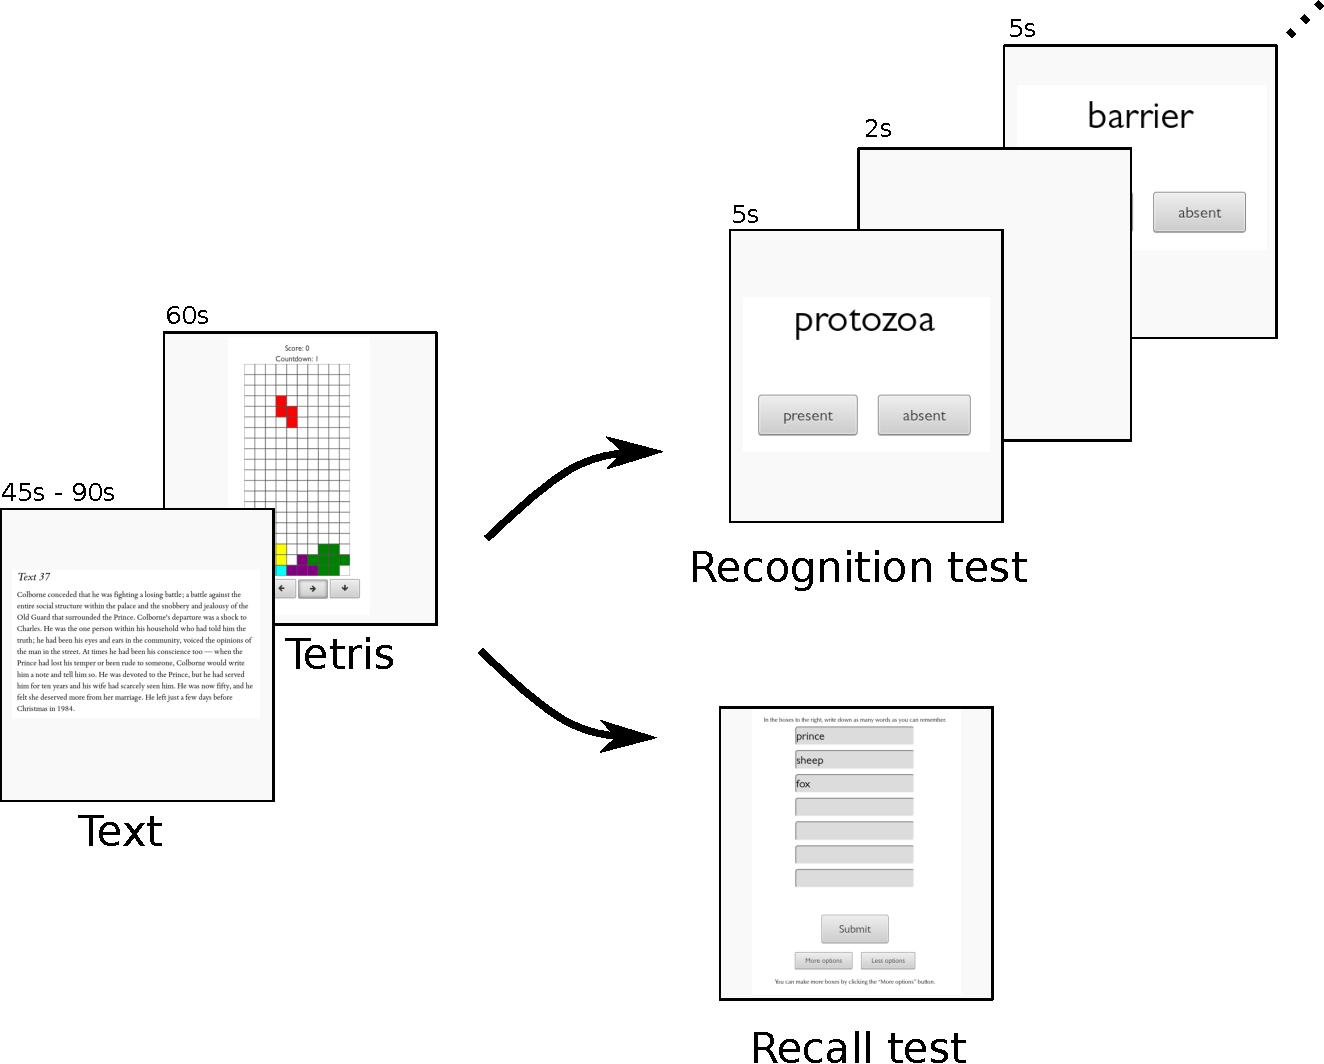
\includegraphics[width=220px]{task_diagram} \end{center}

\end{frame}

\begin{frame}{Recognition memory analysis}
\protect\hypertarget{recognition-memory-analysis}{}

\begin{itemize}
\tightlist
\item
  We analysed the predictions of each of the three models using
  multilevel logistic regression.
\item
  For each model, we modelled the log-odds of recognizing as a
  linear function of the log of
  the model's predictions.
\item
  In each case, this linear function varied randomly by participant, and
  by text, and had random intercept for each word type.
\item
  Each model was evaluated using its \emph{deviance information
  criterion} (\dic), which is a measure of out-of-sample generalization:
\end{itemize}

\begin{longtable}[]{@{}cccc@{}}
\toprule
\begin{minipage}[b]{0.17\columnwidth}\centering
Topic model\strut
\end{minipage} & \begin{minipage}[b]{0.26\columnwidth}\centering
Cooccurrence model\strut
\end{minipage} & \begin{minipage}[b]{0.25\columnwidth}\centering
Association model\strut
\end{minipage} & \begin{minipage}[b]{0.16\columnwidth}\centering
Null model\strut
\end{minipage}\tabularnewline
\midrule
\endhead
\begin{minipage}[t]{0.17\columnwidth}\centering
5232\strut
\end{minipage} & \begin{minipage}[t]{0.26\columnwidth}\centering
5259\strut
\end{minipage} & \begin{minipage}[t]{0.25\columnwidth}\centering
5320\strut
\end{minipage} & \begin{minipage}[t]{0.16\columnwidth}\centering
5352\strut
\end{minipage}\tabularnewline
\bottomrule
\end{longtable}

\end{frame}

\begin{frame}{Recall memory analysis}
\protect\hypertarget{recall-memory-analysis}{}

\begin{itemize}
\tightlist
\item
  We analysed the predictions of each of the three models using
  multilevel multinomial logistic regression.
\item
  For each model, we modelled the probability of recalling a word as
  probability mass function over the vocabulary that is (normalized exponential) linear function
  of the log of the model's predictions.
\item
  In each case, this linear function varied randomly by participant, and
  by text.
\item
  As in the recognition analysis, each model was evaluated using its
  \dic:
\end{itemize}

\begin{longtable}[]{@{}ccc@{}}
\toprule
\begin{minipage}[b]{0.18\columnwidth}\centering
Topic model\strut
\end{minipage} & \begin{minipage}[b]{0.27\columnwidth}\centering
Cooccurrence model\strut
\end{minipage} & \begin{minipage}[b]{0.27\columnwidth}\centering
Association model\strut
\end{minipage}\tabularnewline
\midrule
\endhead
\begin{minipage}[t]{0.18\columnwidth}\centering
23798\strut
\end{minipage} & \begin{minipage}[t]{0.27\columnwidth}\centering
26324\strut
\end{minipage} & \begin{minipage}[t]{0.27\columnwidth}\centering
26825\strut
\end{minipage}\tabularnewline
\bottomrule
\end{longtable}

\end{frame}

\begin{frame}{Conclusion}
\protect\hypertarget{conclusion}{}

\begin{itemize}
\tightlist
\item
  We have proposed a Bayesian account of how we form memories for spoken
  and written language.
\item
  This account models how we use our background knowledge to form
  memories as a process of Bayesian inference of the statistical
  patterns that are inherent in each text, followed by posterior
  predictive inference of the words that are typical of those inferred
  patterns.
\item
  We tested these predictions in a behavioural experiment with 216
  participants.
\item
  The results of the analysis from both the recognition and recall data
  provided strong evidence in favour of the Bayesian model relative to
  non-trivial alternative models.
\end{itemize}

\end{frame}

\begin{frame}{References}
\protect\hypertarget{references}{}

\hypertarget{refs}{}
\leavevmode\hypertarget{ref-bartlett:remembering}{}%
Bartlett, F. C. (1932). \emph{Remembering: A study in experimental and
social psychology}. Cambridge: Cambridge University Press.

\leavevmode\hypertarget{ref-bower:scripts}{}%
Bower, G., Black, J., \& Turner, T. (1979). Scripts in memory for text.
\emph{Cognitive Psychology}, \emph{11}(2), 177--220.

\leavevmode\hypertarget{ref-griffiths:psychrev}{}%
Griffiths, T. L., Steyvers, M., \& Tenenbaum, J. B. (2007). Topics in
semantic representation. \emph{Psychological Review}, \emph{114}(2),
211--244.

\end{frame}

\end{document}
